\documentclass[11pt,a4paper]{article}

% Packages
\usepackage[utf8]{inputenc}
\usepackage[english]{babel}
\usepackage{geometry}
\usepackage{graphicx}
\usepackage{listings}
\usepackage{xcolor}
\usepackage{hyperref}
\usepackage{tcolorbox}
\usepackage{tabularx}
\usepackage{booktabs}
\usepackage{tikz}
\usepackage{forest}
\usepackage{amsmath}
\usepackage{amssymb}
\usepackage{fancyhdr}
\usepackage{titlesec}

% Page geometry
\geometry{
    a4paper,
    left=25mm,
    right=25mm,
    top=30mm,
    bottom=30mm
}

% Header and footer
\pagestyle{fancy}
\fancyhf{}
\fancyhead[L]{embedDIP Architecture Refactoring}
\fancyhead[R]{Version 1.0}
\fancyfoot[C]{\thepage}

% Colors
\definecolor{codegreen}{rgb}{0,0.6,0}
\definecolor{codegray}{rgb}{0.5,0.5,0.5}
\definecolor{codepurple}{rgb}{0.58,0,0.82}
\definecolor{backcolour}{rgb}{0.95,0.95,0.92}
\definecolor{archblue}{RGB}{52,152,219}
\definecolor{boardgreen}{RGB}{46,204,113}
\definecolor{portablegray}{RGB}{149,165,166}

% Code listing style
\lstdefinestyle{cstyle}{
    backgroundcolor=\color{backcolour},
    commentstyle=\color{codegreen},
    keywordstyle=\color{blue}\bfseries,
    numberstyle=\tiny\color{codegray},
    stringstyle=\color{codepurple},
    basicstyle=\ttfamily\footnotesize,
    breakatwhitespace=false,
    breaklines=true,
    captionpos=b,
    keepspaces=true,
    numbers=left,
    numbersep=5pt,
    showspaces=false,
    showstringspaces=false,
    showtabs=false,
    tabsize=4,
    frame=single,
    rulecolor=\color{black}
}

\lstset{style=cstyle}

% Hyperref setup
\hypersetup{
    colorlinks=true,
    linkcolor=blue,
    filecolor=magenta,
    urlcolor=cyan,
    pdftitle={embedDIP Architecture Refactoring Design},
    pdfauthor={embedDIP Development Team},
}

% Title formatting
\titleformat{\section}
    {\normalfont\Large\bfseries\color{blue}}{\thesection}{1em}{}
\titleformat{\subsection}
    {\normalfont\large\bfseries}{\thesubsection}{1em}{}

% Document begins
\begin{document}

% Title Page
\begin{titlepage}
    \centering
    \vspace*{2cm}

    {\Huge\bfseries embedDIP Architecture\\Refactoring Design\\[0.4cm]}

    \vspace{1cm}

    {\Large Separating Architecture from Board Configuration}

    \vspace{2cm}

    {\large
    \textbf{Version:} 1.0\\[0.3cm]
    \textbf{Date:} March 2026\\[0.3cm]
    \textbf{Author:} embedDIP Development Team\\[0.3cm]
    \textbf{Status:} Implementation In Progress
    }

    \vfill

    {\large\textit{A comprehensive guide to restructuring the embedDIP library\\
    for improved code reusability and maintainability}}

    \vspace{1cm}

\end{titlepage}

% Abstract
\begin{abstract}
This document presents a fundamental architectural refactoring of the embedDIP library to separate architecture-specific code (CPU instruction set and optimizations) from board-specific code (hardware peripherals and pin mappings). The current codebase conflates these two distinct layers, limiting code reusability and scalability. We propose a three-layer architecture model: \textbf{Portable Layer} (generic algorithms), \textbf{Architecture Layer} (CPU-specific optimizations), and \textbf{Board Layer} (hardware configuration). This separation enables sharing optimized implementations across multiple boards with the same CPU architecture, simplifies adding new hardware platforms, and improves code maintainability. The document provides detailed implementation guidelines, migration strategies, and testing methodologies for transitioning to the new architecture.

\textbf{Keywords:} Embedded Systems, Software Architecture, Hardware Abstraction, Code Reusability, Digital Image Processing
\end{abstract}

\newpage

% Table of Contents
\tableofcontents

\newpage

% ============================================================================
\section{Executive Summary}
% ============================================================================

\subsection{Overview}

The embedDIP library currently suffers from architectural confusion where code that depends on the CPU architecture (e.g., ARM Cortex-M7 FFT optimizations using CMSIS-DSP) is mixed with code that depends on specific board hardware (e.g., pin mappings, memory addresses for STM32F746G-Discovery). This conflation creates several critical problems:

\begin{itemize}
    \item \textbf{Limited Code Reuse:} ARM Cortex-M7 optimized FFT code cannot be shared between different STM32F7 boards without duplication
    \item \textbf{Duplication Burden:} Adding a new board with the same CPU requires copying architecture-specific code
    \item \textbf{Maintenance Issues:} Bug fixes must be applied to multiple copies of the same architecture code
    \item \textbf{Unclear Dependencies:} Difficult to determine what code depends on CPU vs. hardware
\end{itemize}

\subsection{Proposed Solution}

We propose introducing a \textbf{three-layer architecture} that clearly separates concerns:

\begin{enumerate}
    \item \textbf{Portable Layer} (\texttt{core/}, \texttt{imgproc/}): Generic algorithms that work on any platform
    \item \textbf{Architecture Layer} (\texttt{arch/}): CPU-specific optimizations (FFT, DSP, memory APIs)
    \item \textbf{Board Layer} (\texttt{boards/}): Hardware configuration (pins, peripherals, memory maps)
\end{enumerate}

\begin{tcolorbox}[colback=blue!5!white,colframe=blue!75!black,title=Key Principle]
\textbf{Dependency Flow:} Application $\rightarrow$ Board $\rightarrow$ Architecture $\rightarrow$ Portable

Each layer depends only on layers below it. Architecture code must be independent of board specifics.
\end{tcolorbox}

\subsection{Expected Outcomes}

The refactoring will deliver:

\begin{itemize}
    \item \textbf{Code Reusability:} ARM Cortex-M7 FFT shared across all Cortex-M7 boards (STM32F746, STM32F767, STM32H743, NXP i.MX RT1060)
    \item \textbf{Easy Expansion:} Add new boards with $\sim$100 lines of configuration code instead of duplicating $1000+$ lines
    \item \textbf{Better Testing:} Test architecture features independently from hardware
    \item \textbf{Clear Structure:} Developers immediately understand what code belongs where
\end{itemize}

% ============================================================================
\section{Problem Statement}
% ============================================================================

\subsection{Current Issues}

\subsubsection{Issue 1: Conflated Preprocessor Defines}

The current codebase uses \texttt{TARGET\_BOARD\_STM32F7} to mean both ``ARM Cortex-M7 CPU'' and ``specific STM32F746G-Discovery board''. Consider this example:

\begin{lstlisting}[language=C,caption={Current conflated code structure}]
#ifdef TARGET_BOARD_STM32F7
    // Architecture-specific (works on ANY Cortex-M7)
    #include "arm_math.h"
    arm_cfft_f32(&arm_cfft_sR_f32_len256, buffer, 0, 1);

    // Board-specific (STM32F746G-Discovery only)
    #define SDRAM_BANK_ADDR 0xC0000000
    #define CAMERA_PWR_PIN GPIO_PIN_13
#endif
\end{lstlisting}

\textbf{Problem:} This prevents reusing the FFT code on other ARM Cortex-M7 boards without also hardcoding their specific memory addresses and pin configurations.

\subsubsection{Issue 2: Architecture Code in Board Directories}

The file \texttt{board/stm32f7/board\_stm32f7\_fft.c} contains FFT implementation using ARM CMSIS-DSP:

\begin{lstlisting}[language=C,caption={FFT code misplaced in board directory}]
// File: board/stm32f7/board_stm32f7_fft.c
#include "arm_math.h"

embeddip_status_t fft(const Image *inImg, Image *outImg) {
    // Uses ARM Cortex-M7 DSP instructions
    for (int row = 0; row < N; row++) {
        arm_cfft_f32(&arm_cfft_sR_f32_len256,
                     buffer + row * N * 2, 0, 1);
    }
}
\end{lstlisting}

\textbf{Analysis:} This FFT implementation depends \emph{only} on the ARM Cortex-M7 CPU architecture, not on any specific board hardware. It should be in an architecture directory, not a board directory.

\textbf{Real-World Impact:} To support STM32F767ZI-Nucleo (also Cortex-M7), we must copy this entire file, leading to code duplication and maintenance burden.

\subsubsection{Issue 3: Hardcoded Board Memory Addresses}

\begin{lstlisting}[language=C,caption={Hardcoded board-specific memory addresses}]
// File: board/stm32f7/board_stm32f7_memory.c
#define SDRAM_BANK_ADDR ((uint32_t)0xC0000000)  // Board-specific
#define MEMORY_POOL_SIZE (1024 * 1024 * 8)      // 8MB on this board

static uint8_t *memory_pool =
    ((uint8_t *)SDRAM_BANK_ADDR + FRAMEBUFFER_SIZE);
\end{lstlisting}

\textbf{Problem:} Different STM32F7 boards have different memory configurations:
\begin{itemize}
    \item STM32F746G-Discovery: 8MB SDRAM at 0xC0000000
    \item STM32F767ZI-Nucleo: No external SDRAM (internal RAM only)
    \item STM32H743ZI-Nucleo: 16MB SDRAM at different address
\end{itemize}

Hardcoding these values prevents reusing the memory allocator across boards.

\subsection{Failure Scenarios}

\subsubsection{Scenario A: Adding STM32F767ZI-Nucleo Support}

\textbf{Requirements:}
\begin{itemize}
    \item CPU: ARM Cortex-M7 (identical to STM32F746)
    \item Memory: Internal SRAM only (no SDRAM)
    \item Peripherals: Different GPIO pins, different camera module
\end{itemize}

\textbf{Current Reality:}
\begin{enumerate}
    \item Must copy entire \texttt{board/stm32f7/} directory
    \item Must modify FFT code location (even though FFT algorithm is identical)
    \item Must maintain two separate copies of architecture code
    \item Bug fixes in FFT must be applied twice
\end{enumerate}

\textbf{Expected Behavior:}
\begin{enumerate}
    \item Reuse existing \texttt{arch/arm\_cortex\_m7/} code
    \item Write only \texttt{boards/stm32f767zi\_nucleo/board\_config.h} ($\sim$100 lines)
    \item Automatically inherit all architecture optimizations
\end{enumerate}

This scenario clearly violates the DRY (Don't Repeat Yourself) principle and demonstrates the need for architectural separation.

\subsection{Root Cause Analysis}

The fundamental issue is \textbf{mixing concerns}. The current design conflates three orthogonal questions:

\begin{enumerate}
    \item \textbf{What CPU optimizations are available?} (Architecture concern)
    \begin{itemize}
        \item ARM Cortex-M7: FPU, DSP instructions, CMSIS-DSP library
        \item Xtensa LX6: Dual-core, ESP-DSP library
    \end{itemize}

    \item \textbf{What hardware peripherals exist?} (Board concern)
    \begin{itemize}
        \item OV5640 camera sensor
        \item RK043FN48H LCD display
        \item 8MB SDRAM at 0xC0000000
    \end{itemize}

    \item \textbf{How are they connected?} (Board concern)
    \begin{itemize}
        \item Camera power on GPIO PH13
        \item UART on USART1 (PA9/PA10)
        \item LCD on LTDC peripheral
    \end{itemize}
\end{enumerate}

These are independent concerns that should be separated into distinct layers.

% ============================================================================
\section{Current Architecture Analysis}
% ============================================================================

\subsection{Code Layer Classification}

We performed a comprehensive analysis of the codebase and classified each file by its true layer dependency:

\subsubsection{Portable Code (Platform-Independent)}

\begin{tcolorbox}[colback=portablegray!10!white,colframe=portablegray!75!black,title=Portable Layer Characteristics]
\begin{itemize}
    \item Pure C code with no hardware dependencies
    \item Works on any platform (x86, ARM, Xtensa, RISC-V)
    \item Uses only standard library functions
    \item Contains generic algorithms and data structures
\end{itemize}
\end{tcolorbox}

\textbf{Location:} \texttt{core/}, \texttt{imgproc/}

\textbf{Examples:}
\begin{itemize}
    \item \texttt{core/image.h}: Image data structures
    \item \texttt{core/error.c}: Error handling
    \item \texttt{imgproc/filter.c}: Convolution algorithms
    \item \texttt{imgproc/color.c}: Color space conversions
    \item \texttt{imgproc/histogram.c}: Histogram operations
\end{itemize}

\textbf{Status:} \colorbox{green!30}{Already properly structured} ✓

\subsubsection{Architecture-Specific Code (CPU/ISA-Dependent)}

\begin{tcolorbox}[colback=archblue!10!white,colframe=archblue!75!black,title=Architecture Layer Characteristics]
\begin{itemize}
    \item Uses CPU-specific instructions or libraries
    \item Depends on Instruction Set Architecture (ISA)
    \item Can work on any board with that CPU
    \item Contains optimized implementations
\end{itemize}
\end{tcolorbox}

\textbf{Current Location:} \texttt{board/stm32f7/}, \texttt{board/esp32/} (misplaced)

\textbf{Examples:}

\begin{lstlisting}[language=C,caption={ARM Cortex-M7 FFT (architecture-specific)}]
// Uses ARM CMSIS-DSP library
#include "arm_math.h"
arm_cfft_f32(&arm_cfft_sR_f32_len256, buffer, 0, 1);
\end{lstlisting}

\begin{lstlisting}[language=C,caption={Xtensa LX6 FFT (architecture-specific)}]
// Uses ESP-DSP library
#include "esp_dsp.h"
dsps_fft2r_fc32(buffer, N);
dsps_bit_rev_fc32(buffer, N);
\end{lstlisting}

\textbf{Problem:} Currently mixed with board-specific code \\
\textbf{Solution:} Should be moved to \texttt{arch/} directory

\subsubsection{Board-Specific Code (Hardware-Dependent)}

\begin{tcolorbox}[colback=boardgreen!10!white,colframe=boardgreen!75!black,title=Board Layer Characteristics]
\begin{itemize}
    \item Pin mappings (which GPIO controls what)
    \item Memory layout (SDRAM addresses, sizes)
    \item Peripheral configurations
    \item Hardware initialization sequences
\end{itemize}
\end{tcolorbox}

\textbf{Current Location:} Mixed throughout \texttt{board/}, \texttt{device/}

\textbf{Example:}
\begin{lstlisting}[language=C,caption={Board-specific configuration (STM32F746G-Discovery)}]
// STM32F746G-Discovery specific hardware
#define SDRAM_BANK_ADDR 0xC0000000        // Memory map
#define CAMERA_PWR_PIN GPIO_PIN_13         // Pin wiring
#define CAMERA_PWR_PORT GPIOH              // Pin port
#define BOARD_LCD_WIDTH 480                // LCD specs
#define BOARD_LCD_HEIGHT 272
\end{lstlisting}

\textbf{Problem:} No clear board configuration structure \\
\textbf{Solution:} Should be in \texttt{boards/} directory with standardized config format

\subsection{Dependency Analysis}

Figure~\ref{fig:dependency} shows the current and proposed dependency structures.

\begin{figure}[h]
\centering
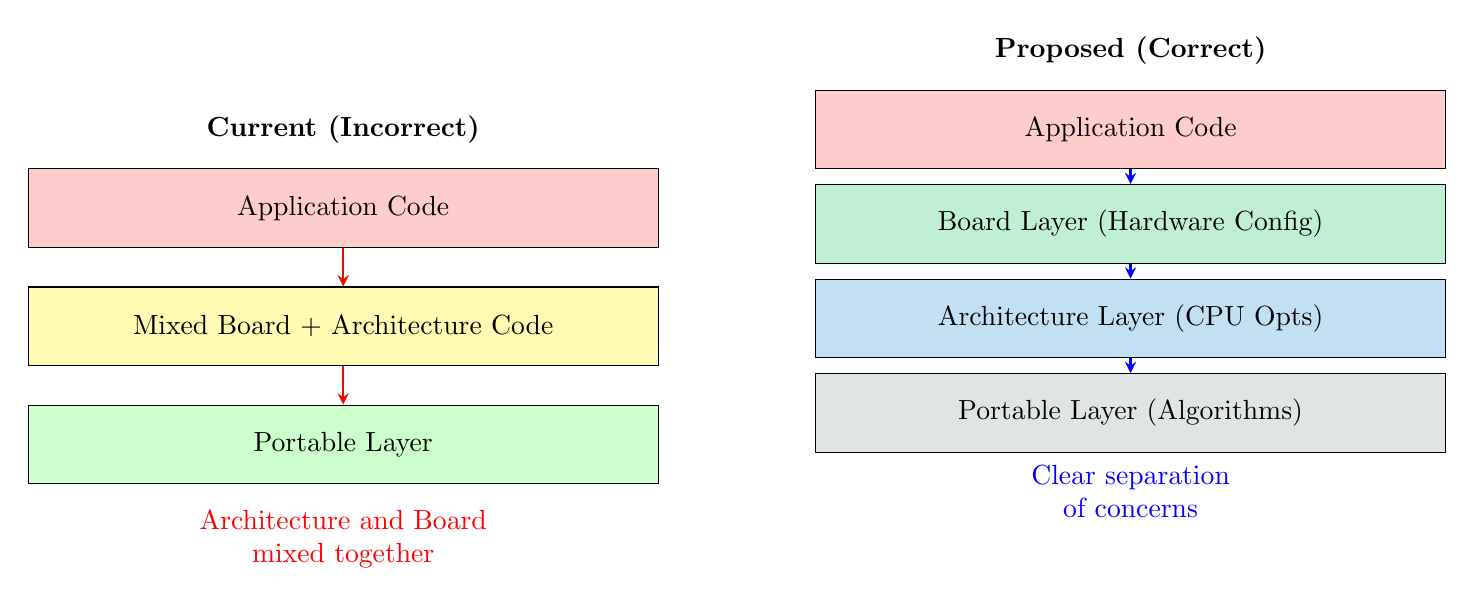
\begin{tikzpicture}[
    layer/.style={rectangle, draw, minimum width=8cm, minimum height=1cm, align=center},
    arrow/.style={->, >=stealth, thick}
]

% Current (left side)
\node[layer, fill=red!20] (app1) at (0,4) {Application Code};
\node[layer, fill=yellow!30] (mixed1) at (0,2.5) {Mixed Board + Architecture Code};
\node[layer, fill=green!20] (port1) at (0,1) {Portable Layer};

\draw[arrow, red] (app1) -- (mixed1);
\draw[arrow, red] (mixed1) -- (port1);

\node at (0,5) {\textbf{Current (Incorrect)}};
\node[red, align=center] at (0,-0.2) {Architecture and Board\\mixed together};

% Proposed (right side)
\node[layer, fill=red!20] (app2) at (10,5) {Application Code};
\node[layer, fill=boardgreen!30] (board2) at (10,3.8) {Board Layer (Hardware Config)};
\node[layer, fill=archblue!30] (arch2) at (10,2.6) {Architecture Layer (CPU Opts)};
\node[layer, fill=portablegray!30] (port2) at (10,1.4) {Portable Layer (Algorithms)};

\draw[arrow, blue] (app2) -- (board2);
\draw[arrow, blue] (board2) -- (arch2);
\draw[arrow, blue] (arch2) -- (port2);

\node at (10,6) {\textbf{Proposed (Correct)}};
\node[blue, align=center] at (10,0.4) {Clear separation\\of concerns};

\end{tikzpicture}
\caption{Dependency structure comparison: current vs. proposed architecture}
\label{fig:dependency}
\end{figure}

\textbf{Key Insight:} Dependencies should flow downward only. Currently, architecture code incorrectly depends on board defines, which violates proper layering principles.

% ============================================================================
\section{Proposed Solution}
% ============================================================================

\subsection{Design Principles}

The proposed architecture adheres to five fundamental software engineering principles:

\begin{enumerate}
    \item \textbf{Separation of Concerns (SoC):} Architecture code must not contain board details
    \item \textbf{Single Responsibility Principle (SRP):} Each layer has one clear purpose
    \item \textbf{Dependency Inversion Principle (DIP):} High-level modules depend on abstractions, not implementations
    \item \textbf{Open/Closed Principle (OCP):} Easy to add new boards without modifying existing code
    \item \textbf{Don't Repeat Yourself (DRY):} Share architecture code across all boards with same CPU
\end{enumerate}

\subsection{Three-Layer Model}

Figure~\ref{fig:threelayer} illustrates the three-layer architecture model.

\begin{figure}[h]
\centering
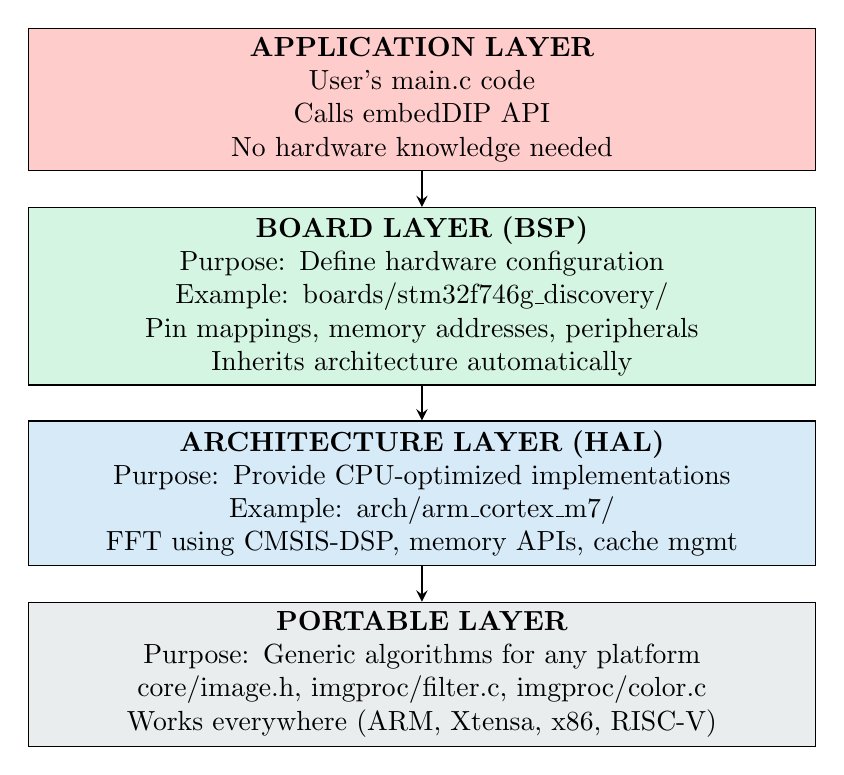
\begin{tikzpicture}[
    layer/.style={rectangle, draw, minimum width=10cm, minimum height=1.8cm, align=center, text width=9cm},
]

% Application
\node[layer, fill=red!20] (app) at (0,7) {
    \textbf{APPLICATION LAYER}\\
    User's main.c code\\
    Calls embedDIP API\\
    No hardware knowledge needed
};

% Board
\node[layer, fill=boardgreen!20] (board) at (0,4.5) {
    \textbf{BOARD LAYER (BSP)}\\
    Purpose: Define hardware configuration\\
    Example: boards/stm32f746g\_discovery/\\
    Pin mappings, memory addresses, peripherals\\
    Inherits architecture automatically
};

% Architecture
\node[layer, fill=archblue!20] (arch) at (0,2) {
    \textbf{ARCHITECTURE LAYER (HAL)}\\
    Purpose: Provide CPU-optimized implementations\\
    Example: arch/arm\_cortex\_m7/\\
    FFT using CMSIS-DSP, memory APIs, cache mgmt
};

% Portable
\node[layer, fill=portablegray!20] (port) at (0,-0.3) {
    \textbf{PORTABLE LAYER}\\
    Purpose: Generic algorithms for any platform\\
    core/image.h, imgproc/filter.c, imgproc/color.c\\
    Works everywhere (ARM, Xtensa, x86, RISC-V)
};

% Arrows
\draw[->, >=stealth, thick] (app) -- (board);
\draw[->, >=stealth, thick] (board) -- (arch);
\draw[->, >=stealth, thick] (arch) -- (port);

\end{tikzpicture}
\caption{Three-layer architecture model with clear separation of concerns}
\label{fig:threelayer}
\end{figure}

\subsection{Layer Responsibilities}

\subsubsection{Layer 1: Portable (core/, imgproc/)}

\textbf{Responsibility:} Provide generic, platform-independent functionality

\textbf{Rules:}
\begin{itemize}
    \item[✓] Use only standard C/C++ library
    \item[✓] Define abstract interfaces
    \item[✗] No hardware-specific code
    \item[✗] No CPU-specific optimizations
\end{itemize}

\textbf{Example:}
\begin{lstlisting}[language=C,caption={Abstract memory interface (portable layer)}]
// core/memory_manager.h
void* memory_alloc(size_t size);  // Abstract interface
void memory_free(void* ptr);
\end{lstlisting}

\subsubsection{Layer 2: Architecture (arch/)}

\textbf{Responsibility:} Implement CPU-specific optimizations

\textbf{Rules:}
\begin{itemize}
    \item[✓] Use CPU instruction set (NEON, DSP extensions)
    \item[✓] Use architecture-specific libraries (CMSIS-DSP, ESP-DSP)
    \item[✓] Can vary by CPU model (Cortex-M4 vs M7)
    \item[✗] No board-specific addresses or pins
    \item[✗] No peripheral initialization
\end{itemize}

\textbf{Example:}
\begin{lstlisting}[language=C,caption={ARM Cortex-M7 FFT implementation (architecture layer)}]
// arch/arm_cortex_m7/arch_fft.c
#include "arm_math.h"

int arch_fft_2d(const float *input, float *output,
                int width, int height) {
    // Uses Cortex-M7 DSP instructions
    for (int row = 0; row < height; row++) {
        arm_cfft_f32(&arm_cfft_sR_f32_len256,
                     output + row * width * 2, 0, 1);
    }
    return 0;
}
\end{lstlisting}

\subsubsection{Layer 3: Board (boards/)}

\textbf{Responsibility:} Define hardware configuration

\textbf{Rules:}
\begin{itemize}
    \item[✓] Define pin mappings
    \item[✓] Define memory layout (addresses, sizes)
    \item[✓] Configure peripherals
    \item[✓] Specify which architecture to use
    \item[✗] No algorithm implementations
    \item[✗] No CPU-specific optimizations
\end{itemize}

\textbf{Example:}
\begin{lstlisting}[language=C,caption={STM32F746G-Discovery configuration (board layer)}]
// boards/stm32f746g_discovery/board_config.h
#ifndef BOARD_CONFIG_H
#define BOARD_CONFIG_H

// Specify architecture (pulls in arch layer automatically)
#define ARCH_ARM_CORTEX_M7 1

// Board identification
#define BOARD_NAME "STM32F746G-Discovery"

// Memory configuration
#define BOARD_SDRAM_BASE 0xC0000000
#define BOARD_SDRAM_SIZE (8 * 1024 * 1024)  // 8MB

// Pin mappings
#define BOARD_CAMERA_PWR_PIN GPIO_PIN_13
#define BOARD_CAMERA_PWR_PORT GPIOH

// Available peripherals
#define BOARD_HAS_CAMERA_OV5640 1
#define BOARD_HAS_LCD_RK043FN48H 1

#endif
\end{lstlisting}

% ============================================================================
\section{Directory Structure}
% ============================================================================

The proposed directory structure provides clear separation between layers:

\begin{lstlisting}[basicstyle=\ttfamily\small,frame=single]
embedDIP/
|
+-- core/                    # Portable Layer (no changes)
|   +-- image.h              # Image data structures
|   +-- error.c              # Error handling
|   +-- memory_manager.h     # Abstract memory interface
|
+-- imgproc/                 # Portable Layer (no changes)
|   +-- color.c              # Color conversions
|   +-- filter.c             # Convolution algorithms
|   +-- histogram.c          # Histogram operations
|   +-- pixel.c              # Pixel manipulation
|
+-- arch/                    # NEW: Architecture Layer
|   +-- arch.h               # Common interface
|   |
|   +-- arm_cortex_m7/       # ARM Cortex-M7 implementation
|   |   +-- arch_config.h    # Architecture capabilities
|   |   +-- arch_fft.c       # FFT using CMSIS-DSP
|   |   +-- arch_memory.c    # Memory allocation
|   |   +-- arch_init.c      # CPU initialization
|   |
|   +-- arm_cortex_m4/       # ARM Cortex-M4 implementation
|   |   +-- arch_config.h
|   |   +-- arch_fft.c       # Single-precision FPU
|   |   +-- arch_memory.c
|   |
|   +-- xtensa_lx6/          # Xtensa LX6 (ESP32)
|   |   +-- arch_config.h
|   |   +-- arch_fft.cpp     # FFT using ESP-DSP
|   |   +-- arch_memory.cpp  # PSRAM allocation
|   |
|   +-- host/                # x86/x64 for testing
|       +-- arch_fft.c       # Software FFT
|       +-- arch_memory.c    # malloc/free wrapper
|
+-- boards/                  # NEW: Board Support Packages
|   +-- stm32f746g_discovery/
|   |   +-- board_config.h   # Hardware configuration
|   |   +-- board_init.c     # Board initialization
|   |   +-- README.md        # Board documentation
|   |
|   +-- stm32f767zi_nucleo/
|   |   +-- board_config.h   # Different pins, no SDRAM
|   |   +-- board_init.c
|   |
|   +-- esp32_cam/
|   |   +-- board_config.h
|   |   +-- board_init.cpp
|   |
|   +-- host/
|       +-- board_config.h
|       +-- board_init.c
|
+-- device/                  # Device drivers (can be shared)
|   +-- camera/
|   |   +-- ov5640/          # Generic OV5640 driver
|   |   +-- ov2640/          # Generic OV2640 driver
|   +-- display/
|   +-- serial/
|
+-- docs/
|   +-- ARCHITECTURE_REFACTORING.md
|   +-- ARCHITECTURE_REFACTORING.tex  # This document
|
+-- CMakeLists.txt           # Updated build system
\end{lstlisting}

% ============================================================================
\section{Implementation Strategy}
% ============================================================================

\subsection{Architecture Interface Definition}

All architectures must implement a common interface defined in \texttt{arch/arch.h}:

\begin{lstlisting}[language=C,caption={Common architecture interface}]
#ifndef EMBEDDIP_ARCH_H
#define EMBEDDIP_ARCH_H

#include <stddef.h>
#include <stdint.h>

// Memory Management Interface
void arch_memory_init(void);
void* arch_memory_alloc(size_t size);
void arch_memory_free(void* ptr);
void* arch_memory_realloc(void* ptr, size_t new_size);

// FFT Interface
int arch_fft_2d(const float* input, float* output,
                int width, int height);
int arch_ifft_2d(const float* input, float* output,
                 int width, int height);

// Initialization
void arch_init(void);

#endif // EMBEDDIP_ARCH_H
\end{lstlisting}

\subsection{Build System Configuration}

The CMake build system maps boards to architectures automatically:

\begin{lstlisting}[language=bash,caption={CMake board selection}]
# User selects BOARD (not architecture)
cmake -B build -DEMBEDDIP_BOARD=STM32F746G_DISCOVERY

# Build system determines architecture automatically
# STM32F746G_DISCOVERY -> ARM_CORTEX_M7
\end{lstlisting}

Configuration mapping in \texttt{cmake/BoardConfigs.cmake}:

\begin{lstlisting}[language=bash,caption={Board to architecture mapping}]
if(EMBEDDIP_BOARD STREQUAL "STM32F746G_DISCOVERY")
    set(EMBEDDIP_ARCH "ARM_CORTEX_M7")
    set(ARCH_SOURCES
        arch/arm_cortex_m7/arch_fft.c
        arch/arm_cortex_m7/arch_memory.c
    )
    set(BOARD_SOURCES
        boards/stm32f746g_discovery/board_init.c
    )
endif()
\end{lstlisting}

% ============================================================================
\section{Migration Plan}
% ============================================================================

\subsection{Seven-Week Implementation Timeline}

\begin{table}[h]
\centering
\begin{tabularx}{\textwidth}{|l|X|}
\hline
\textbf{Week} & \textbf{Tasks} \\
\hline
1 & \textbf{Preparation:} Create directory structure, interface headers, backup code \\
\hline
2 & \textbf{Architecture Layer:} Move ARM Cortex-M7 FFT/memory to arch/, test independently \\
\hline
3 & \textbf{Architecture Layer:} Move Xtensa LX6 FFT/memory to arch/, test independently \\
\hline
4 & \textbf{Board Configurations:} Extract board configs, create board\_init.c files \\
\hline
5 & \textbf{Build System:} Update CMakeLists.txt, test all board builds \\
\hline
6 & \textbf{Testing:} Unit tests, integration tests, hardware validation \\
\hline
7 & \textbf{Finalization:} Documentation, cleanup, remove old code \\
\hline
\end{tabularx}
\caption{Seven-week migration timeline}
\end{table}

\subsection{Adding New Boards After Refactoring}

After refactoring, adding a new board becomes trivial:

\begin{tcolorbox}[colback=green!10!white,colframe=green!75!black,title=Example: Adding STM32F767ZI-Nucleo]

\textbf{Step 1:} Create board directory
\begin{lstlisting}[language=bash]
mkdir -p boards/stm32f767zi_nucleo
\end{lstlisting}

\textbf{Step 2:} Create board\_config.h ($\sim$50 lines)
\begin{lstlisting}[language=C]
#define ARCH_ARM_CORTEX_M7 1  // Inherit architecture
#define BOARD_SRAM_BASE 0x20000000
#define BOARD_SRAM_SIZE (512 * 1024)
// No SDRAM on this board
\end{lstlisting}

\textbf{Step 3:} Create board\_init.c ($\sim$50 lines)
\begin{lstlisting}[language=C]
void board_init(void) {
    HAL_Init();
    SystemClock_Config();
    arch_init();  // Calls inherited architecture
}
\end{lstlisting}

\textbf{Step 4:} Add to CMake
\begin{lstlisting}[language=bash]
elseif(EMBEDDIP_BOARD STREQUAL "STM32F767ZI_NUCLEO")
    set(EMBEDDIP_ARCH "ARM_CORTEX_M7")  # Reuse existing!
    ...
endif()
\end{lstlisting}

\textbf{Total new code:} $\sim$100 lines \\
\textbf{Code reused:} 1000+ lines of ARM Cortex-M7 FFT and memory code
\end{tcolorbox}

% ============================================================================
\section{Benefits Analysis}
% ============================================================================

\subsection{Quantitative Benefits}

Table~\ref{tab:benefits} compares code metrics before and after refactoring:

\begin{table}[h]
\centering
\begin{tabularx}{\textwidth}{|l|X|X|}
\hline
\textbf{Metric} & \textbf{Before} & \textbf{After} \\
\hline
Lines to add new board & $\sim$1200 (copy \& modify) & $\sim$100 (config only) \\
\hline
FFT code copies & 1 per board & 1 per architecture \\
\hline
Bug fix locations & Multiple files & Single arch file \\
\hline
Build configurations & Platform-based & Board + arch \\
\hline
Test independence & Cannot test arch alone & Can test each layer \\
\hline
\end{tabularx}
\caption{Quantitative comparison of architectural approaches}
\label{tab:benefits}
\end{table}

\subsection{Qualitative Benefits}

\begin{enumerate}
    \item \textbf{Developer Experience:} Clear structure makes onboarding easier
    \item \textbf{Code Review:} Reviewers immediately understand layer responsibilities
    \item \textbf{Testing:} Can mock boards and test architectures independently
    \item \textbf{Documentation:} Natural organization for API documentation
    \item \textbf{Portability:} Easy to add support for new CPU architectures
\end{enumerate}

\subsection{Risk Mitigation}

\begin{table}[h]
\centering
\begin{tabularx}{\textwidth}{|l|l|X|}
\hline
\textbf{Risk} & \textbf{Impact} & \textbf{Mitigation} \\
\hline
Breaking existing code & High & Incremental migration, backward compatibility \\
\hline
Performance regression & Medium & Benchmark before/after, verify assembly \\
\hline
Build system errors & Medium & Test all boards after each change \\
\hline
Developer confusion & Low & Training, documentation, code reviews \\
\hline
\end{tabularx}
\caption{Risk analysis and mitigation strategies}
\end{table}

% ============================================================================
\section{Testing Strategy}
% ============================================================================

\subsection{Testing Hierarchy}

Testing follows the three-layer structure:

\begin{enumerate}
    \item \textbf{Unit Tests:} Test each architecture implementation independently
    \item \textbf{Integration Tests:} Test interaction between layers
    \item \textbf{Hardware Tests:} Validate on real boards
    \item \textbf{Regression Tests:} Ensure identical results to pre-refactoring
\end{enumerate}

\subsection{Architecture Layer Unit Tests}

\begin{lstlisting}[language=C,caption={Example architecture unit test}]
// tests/test_arch_fft.c
void test_arm_cortex_m7_fft(void) {
    // Mock board config
    #define BOARD_MEMORY_POOL_BASE 0x20000000
    #define BOARD_MEMORY_POOL_SIZE (512 * 1024)

    float input[256 * 256];
    float output[256 * 256 * 2];

    // Initialize test pattern
    for (int i = 0; i < 256 * 256; i++) {
        input[i] = (float)i;
    }

    // Run FFT
    int result = arch_fft_2d(input, output, 256, 256);
    assert(result == 0);

    // Verify DC component
    float dc_real = output[0];
    float expected_dc = (256*256) * (256*256-1) / 2.0f;
    assert(fabs(dc_real - expected_dc) < 1e-3);
}
\end{lstlisting}

\subsection{Regression Testing}

Ensure refactored code produces identical results:

\begin{lstlisting}[language=Python,caption={Python regression test}]
# tests/regression_test.py
def test_fft_output_unchanged():
    # Load pre-refactoring output (golden reference)
    golden = np.load('tests/golden/fft_256x256.npy')

    # Run post-refactoring code
    result = run_embedDIP_fft('tests/inputs/test.raw')

    # Compare with tight tolerance
    np.testing.assert_allclose(result, golden,
                               rtol=1e-5, atol=1e-8)
\end{lstlisting}

% ============================================================================
\section{Conclusion}
% ============================================================================

This document has presented a comprehensive architectural refactoring of the embedDIP library to separate architecture-specific code (CPU optimizations) from board-specific code (hardware configuration). The proposed three-layer model provides:

\begin{itemize}
    \item \textbf{Clear Separation:} Architecture, board, and portable code in distinct layers
    \item \textbf{Code Reuse:} Share ARM Cortex-M7 FFT across all Cortex-M7 boards
    \item \textbf{Easy Expansion:} Add new boards with minimal code ($\sim$100 lines)
    \item \textbf{Better Testing:} Test each layer independently
    \item \textbf{Maintainability:} Bug fixes apply automatically to all boards with same architecture
\end{itemize}

The refactoring follows established software engineering principles (SoC, SRP, DIP, OCP, DRY) and provides a solid foundation for supporting diverse hardware platforms while maintaining a unified codebase.

\subsection{Next Steps}

\begin{enumerate}
    \item \textbf{Review \& Approval:} Stakeholder review of this design document
    \item \textbf{Prototype:} Implement one complete example (STM32F746G-Discovery)
    \item \textbf{Validation:} Test on hardware, verify performance
    \item \textbf{Full Migration:} Follow seven-week implementation plan
    \item \textbf{Documentation:} Update developer guides and API documentation
\end{enumerate}

\subsection{Success Criteria}

The refactoring will be considered successful when:

\begin{itemize}
    \item All existing boards compile and run with identical functionality
    \item No performance regression ($<$5\% variance)
    \item Adding STM32F767ZI-Nucleo requires $<$150 lines of new code
    \item Architecture layer can be tested without hardware
    \item All unit and integration tests pass
\end{itemize}

% ============================================================================
% References
% ============================================================================
\newpage
\section*{References}

\begin{thebibliography}{9}

\bibitem{martin2017}
Robert C. Martin,
\textit{Clean Architecture: A Craftsman's Guide to Software Structure and Design},
Prentice Hall, 2017.

\bibitem{gamma1994}
Erich Gamma, Richard Helm, Ralph Johnson, John Vlissides,
\textit{Design Patterns: Elements of Reusable Object-Oriented Software},
Addison-Wesley, 1994.

\bibitem{cmsis}
ARM,
\textit{CMSIS-DSP Software Library},
\url{https://arm-software.github.io/CMSIS_5/DSP/html/index.html}, 2024.

\bibitem{espdsp}
Espressif Systems,
\textit{ESP-DSP Library Documentation},
\url{https://docs.espressif.com/projects/esp-dsp/}, 2024.

\bibitem{embedded}
Elecia White,
\textit{Making Embedded Systems: Design Patterns for Great Software},
O'Reilly Media, 2011.

\end{thebibliography}

% ============================================================================
% Appendix
% ============================================================================
\newpage
\appendix

\section{Glossary}

\begin{description}
    \item[Architecture] The CPU instruction set and features (ARM Cortex-M7, Xtensa LX6). Code that uses CPU-specific instructions or optimized libraries.

    \item[Board / BSP] Board Support Package - specific hardware platform with defined peripherals, pins, and memory layout.

    \item[Portable Code] Generic algorithms that work on any platform without modification.

    \item[HAL] Hardware Abstraction Layer - interface that hides hardware differences.

    \item[CMSIS-DSP] ARM Cortex Microcontroller Software Interface Standard - Digital Signal Processing library.

    \item[ESP-DSP] Espressif Digital Signal Processing library for Xtensa processors.

    \item[ISA] Instruction Set Architecture - the set of instructions a CPU can execute.

    \item[FPU] Floating-Point Unit - hardware accelerator for floating-point operations.

    \item[DCMI] Digital Camera Interface - STM32 peripheral for camera sensors.

    \item[LTDC] LCD-TFT Display Controller - STM32 peripheral for LCD displays.
\end{description}

\section{Complete Board Configuration Example}

\begin{lstlisting}[language=C,caption={Complete board\_config.h example}]
// boards/stm32f746g_discovery/board_config.h
#ifndef BOARD_CONFIG_H
#define BOARD_CONFIG_H

// Architecture selection
#define ARCH_ARM_CORTEX_M7 1
#include "arch/arm_cortex_m7/arch_config.h"

// Board identification
#define BOARD_NAME "STM32F746G-Discovery"
#define BOARD_VENDOR "STMicroelectronics"
#define BOARD_FAMILY "STM32F7"

// Memory configuration
#define BOARD_FLASH_BASE 0x08000000
#define BOARD_FLASH_SIZE (1024 * 1024)
#define BOARD_SRAM_BASE 0x20000000
#define BOARD_SRAM_SIZE (320 * 1024)
#define BOARD_SDRAM_BASE 0xC0000000
#define BOARD_SDRAM_SIZE (8 * 1024 * 1024)

// Framebuffer allocation
#define BOARD_FRAMEBUFFER_BASE BOARD_SDRAM_BASE
#define BOARD_FRAMEBUFFER_SIZE (480 * 272 * 4)

// Dynamic memory pool
#define BOARD_MEMORY_POOL_BASE \
    (BOARD_FRAMEBUFFER_BASE + BOARD_FRAMEBUFFER_SIZE)
#define BOARD_MEMORY_POOL_SIZE \
    (BOARD_SDRAM_SIZE - BOARD_FRAMEBUFFER_SIZE)

// Peripheral availability
#define BOARD_HAS_CAMERA 1
#define BOARD_CAMERA_TYPE "OV5640"
#define BOARD_CAMERA_INTERFACE "DCMI"

#define BOARD_HAS_LCD 1
#define BOARD_LCD_TYPE "RK043FN48H"
#define BOARD_LCD_WIDTH 480
#define BOARD_LCD_HEIGHT 272

// Pin mappings
#define BOARD_CAMERA_PWR_PIN GPIO_PIN_13
#define BOARD_CAMERA_PWR_PORT GPIOH
#define BOARD_UART_TX_PIN GPIO_PIN_9
#define BOARD_UART_TX_PORT GPIOA

// Clock configuration
#define BOARD_CPU_CLOCK_HZ 216000000

#endif // BOARD_CONFIG_H
\end{lstlisting}

\end{document}
